%EKG-7 Realisierung/Gehäuse
\subsection{Gehäuse}
Dieses Unterkapitel behandelt die Konstruktion des Gehäuses für das gesamte EKG Projekt. Zur Modellierung der 3D-Druck Teile wurde die Open Source Software Blender \cite{Blender} verwendet. Um bereits während des Designs die Position und Größe der verschiedenen Elektronik Komponenten zu visualisieren, wurden diese als externe .step-Dateien importiert und im Gehäuse an der passenden Position platziert.

\begin{table}[h]
\centering
\caption{Gehäuse Merkmale}
\begin{tabular}[h]{l|l|l|l|l}
		& Außenbreite & Außenlänge & Außenhöhe & Produktgewicht \\
\hline
Maße 	& 120 mm & 100 mm & 25 mm & 235 g \\
\end{tabular}
\end{table}

Das Display ist mit vier Stahlstützen oberhalb der Platine befestigt und ermöglicht so ein besonders kompaktes Design (Abbildung \ref{case_display}) des EKG-Gerätes. Das Langloch zum Tauschen der SD-Karte wird im fertigen Zustand durch eine Gummi-Membran verschlossen und schützt so die inneren Komponenten vor Verschmutzung. Der Deckel wird mit vier M3x18 Schlitzschrauben befestigt und kann somit zum Laden des Akkus abgenommen werden. \\
Die gerenderten Bilder geben einen Einblick in das Konzept und Design der Box (Abbildung \ref{case_no_display1} und \ref{case_no_display2}) sowie des Deckels (Abbildung \ref{case_closed}).

\begin{figure}
	\begin{subfigure}[t]{0.49\textwidth}
		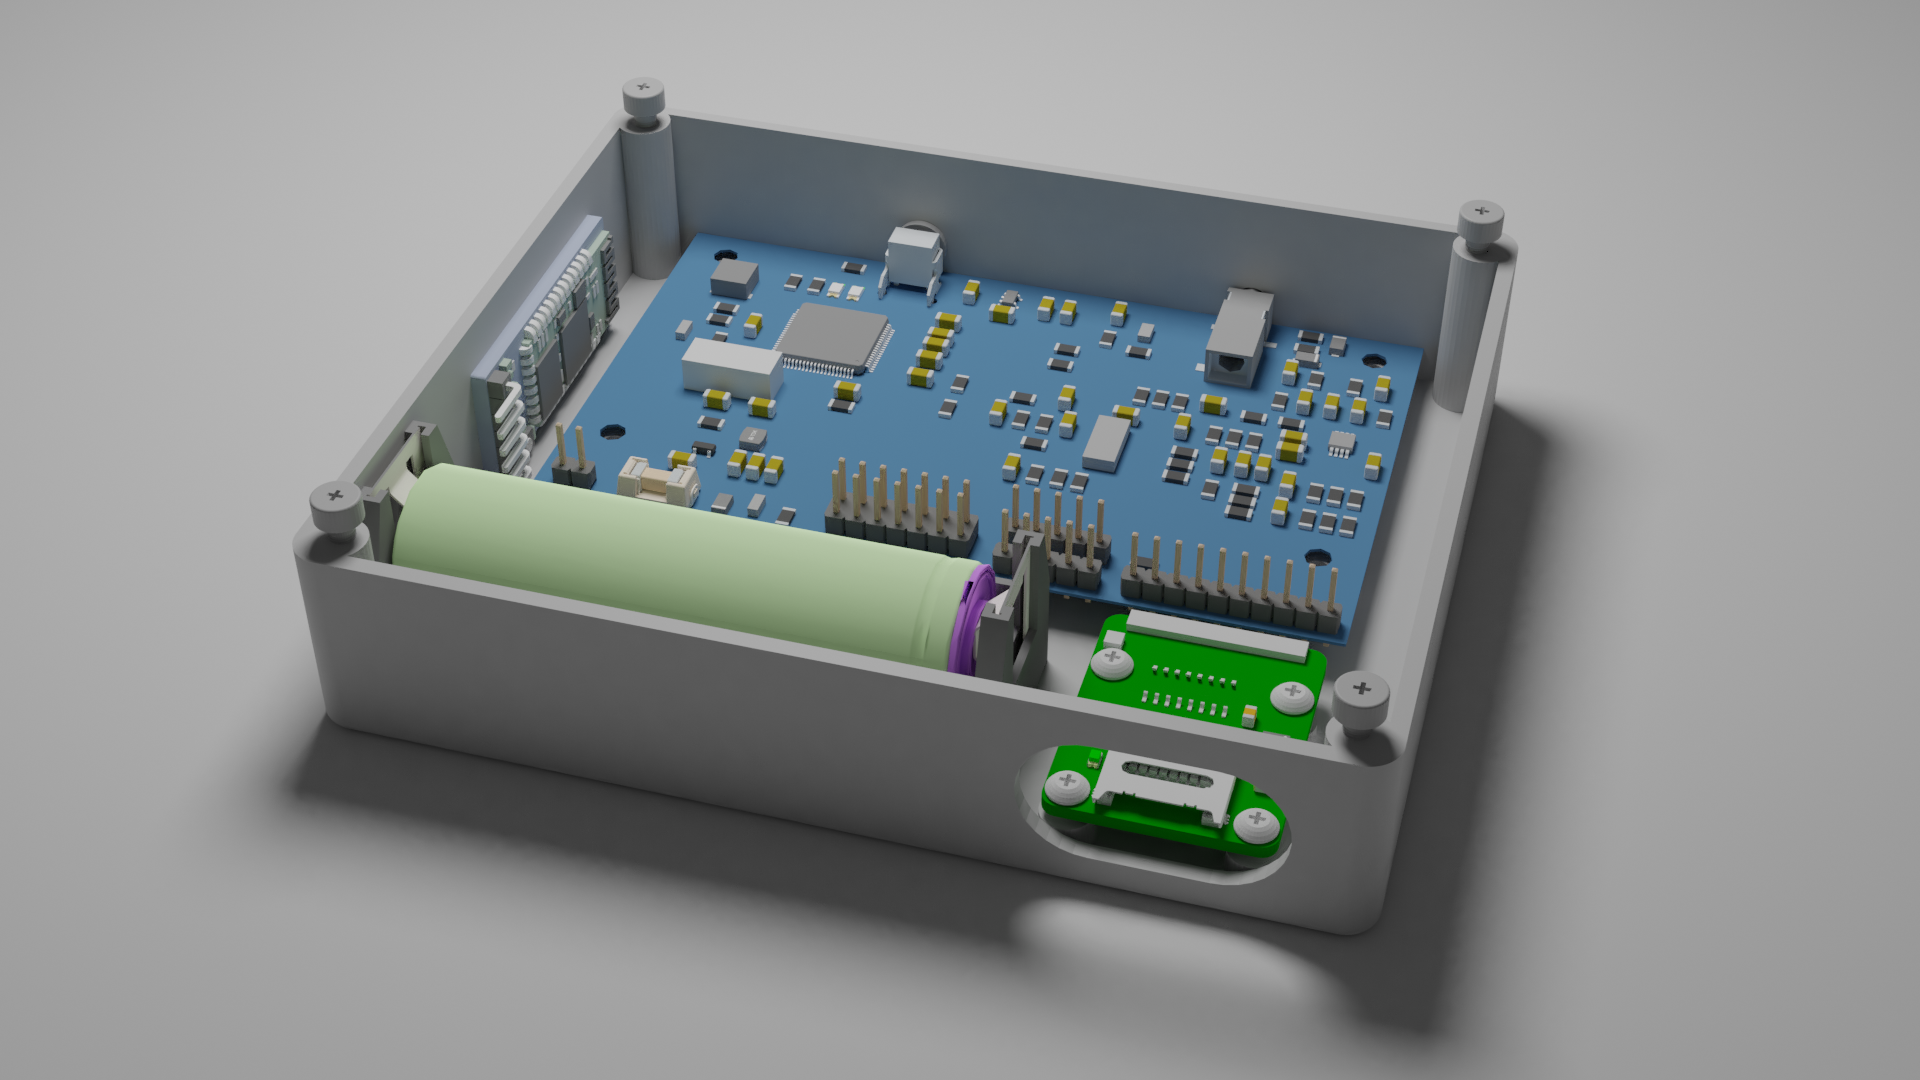
\includegraphics[width=\textwidth]{case_no_display.png}
		\caption{Vorderseite Gehäuse ohne Display}
		\label{case_no_display1}
	\end{subfigure}\hfill%
	\begin{subfigure}[t]{0.49\textwidth}
		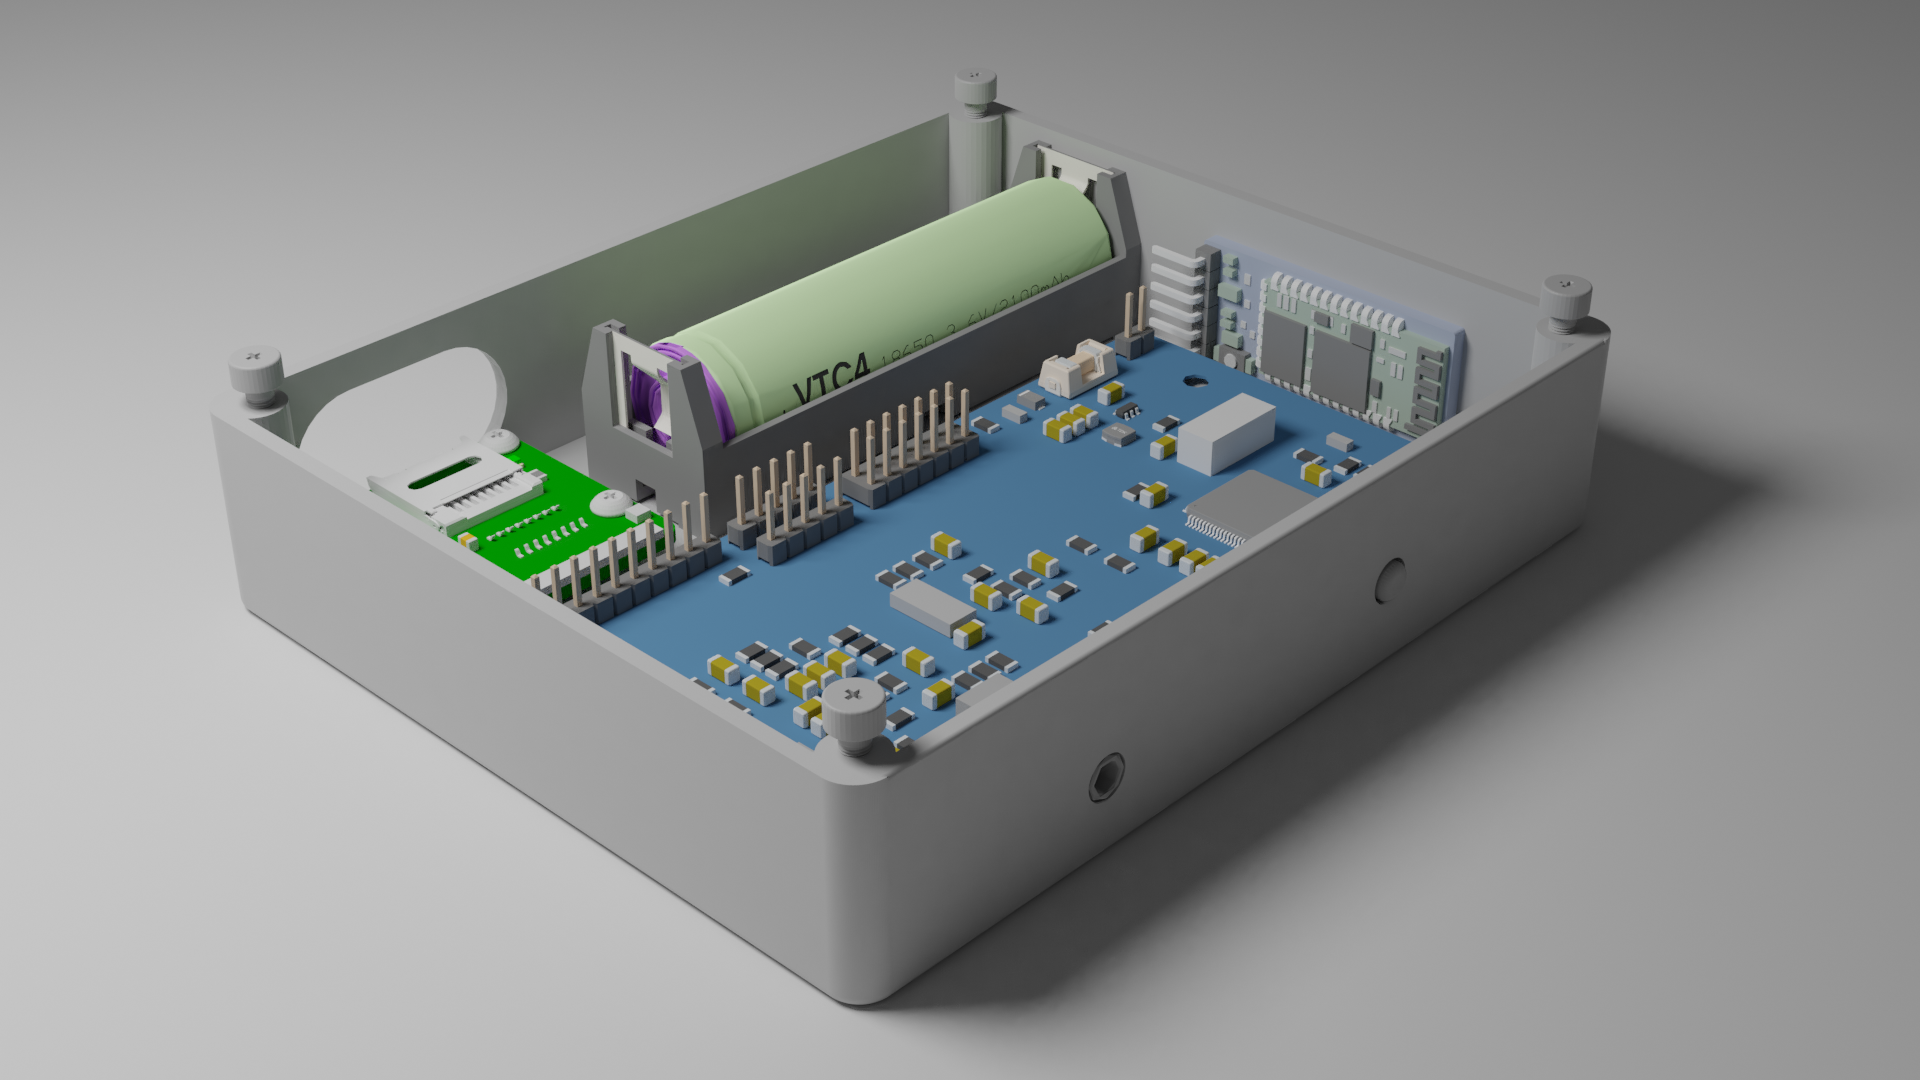
\includegraphics[width=\textwidth]{case_no_display_2.png}
		\caption{Rückseite Gehäuse ohne Display}
		\label{case_no_display2}
	\end{subfigure}\\[5pt]%
	
	\begin{subfigure}[t]{0.49\textwidth}
		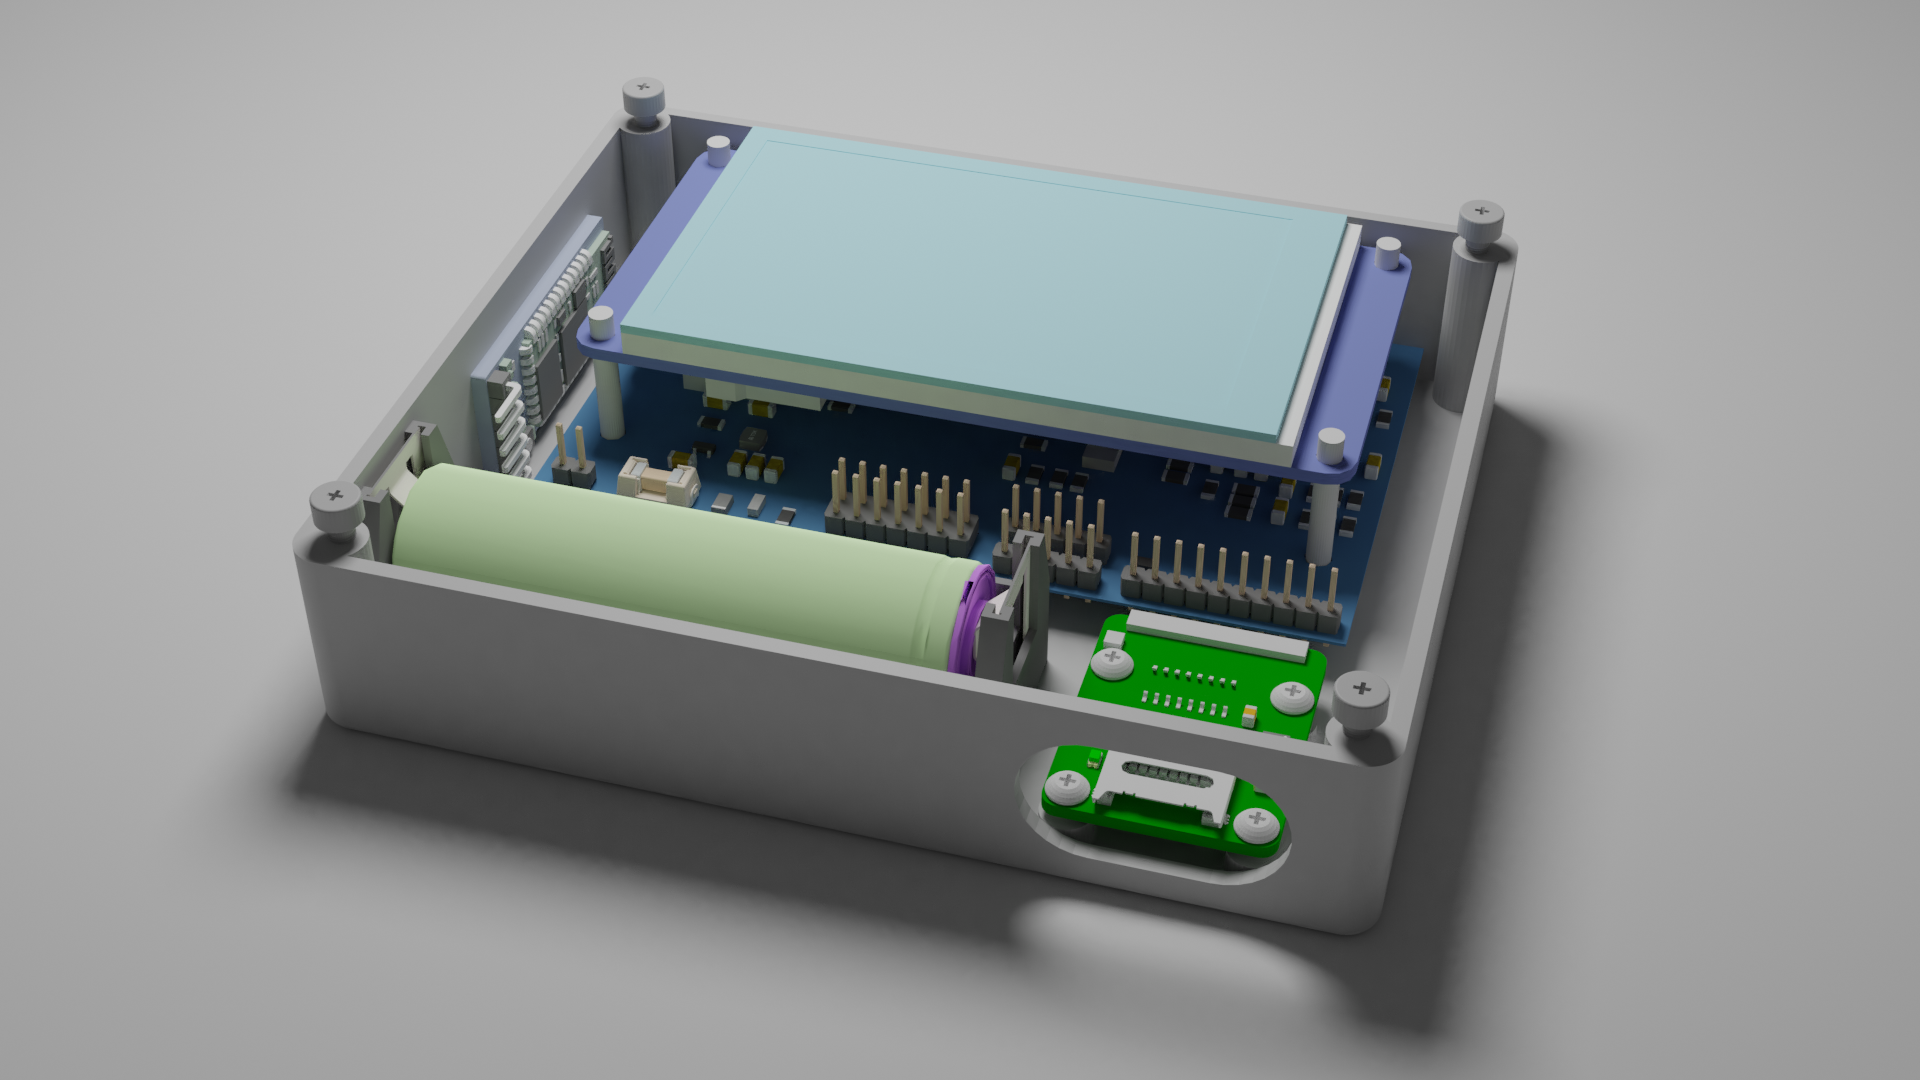
\includegraphics[width=\textwidth]{case_display.png}
		\caption{Gehäuse mit Display}
		\label{case_display}
	\end{subfigure}\hfill%
	\begin{subfigure}[t]{0.49\textwidth}
		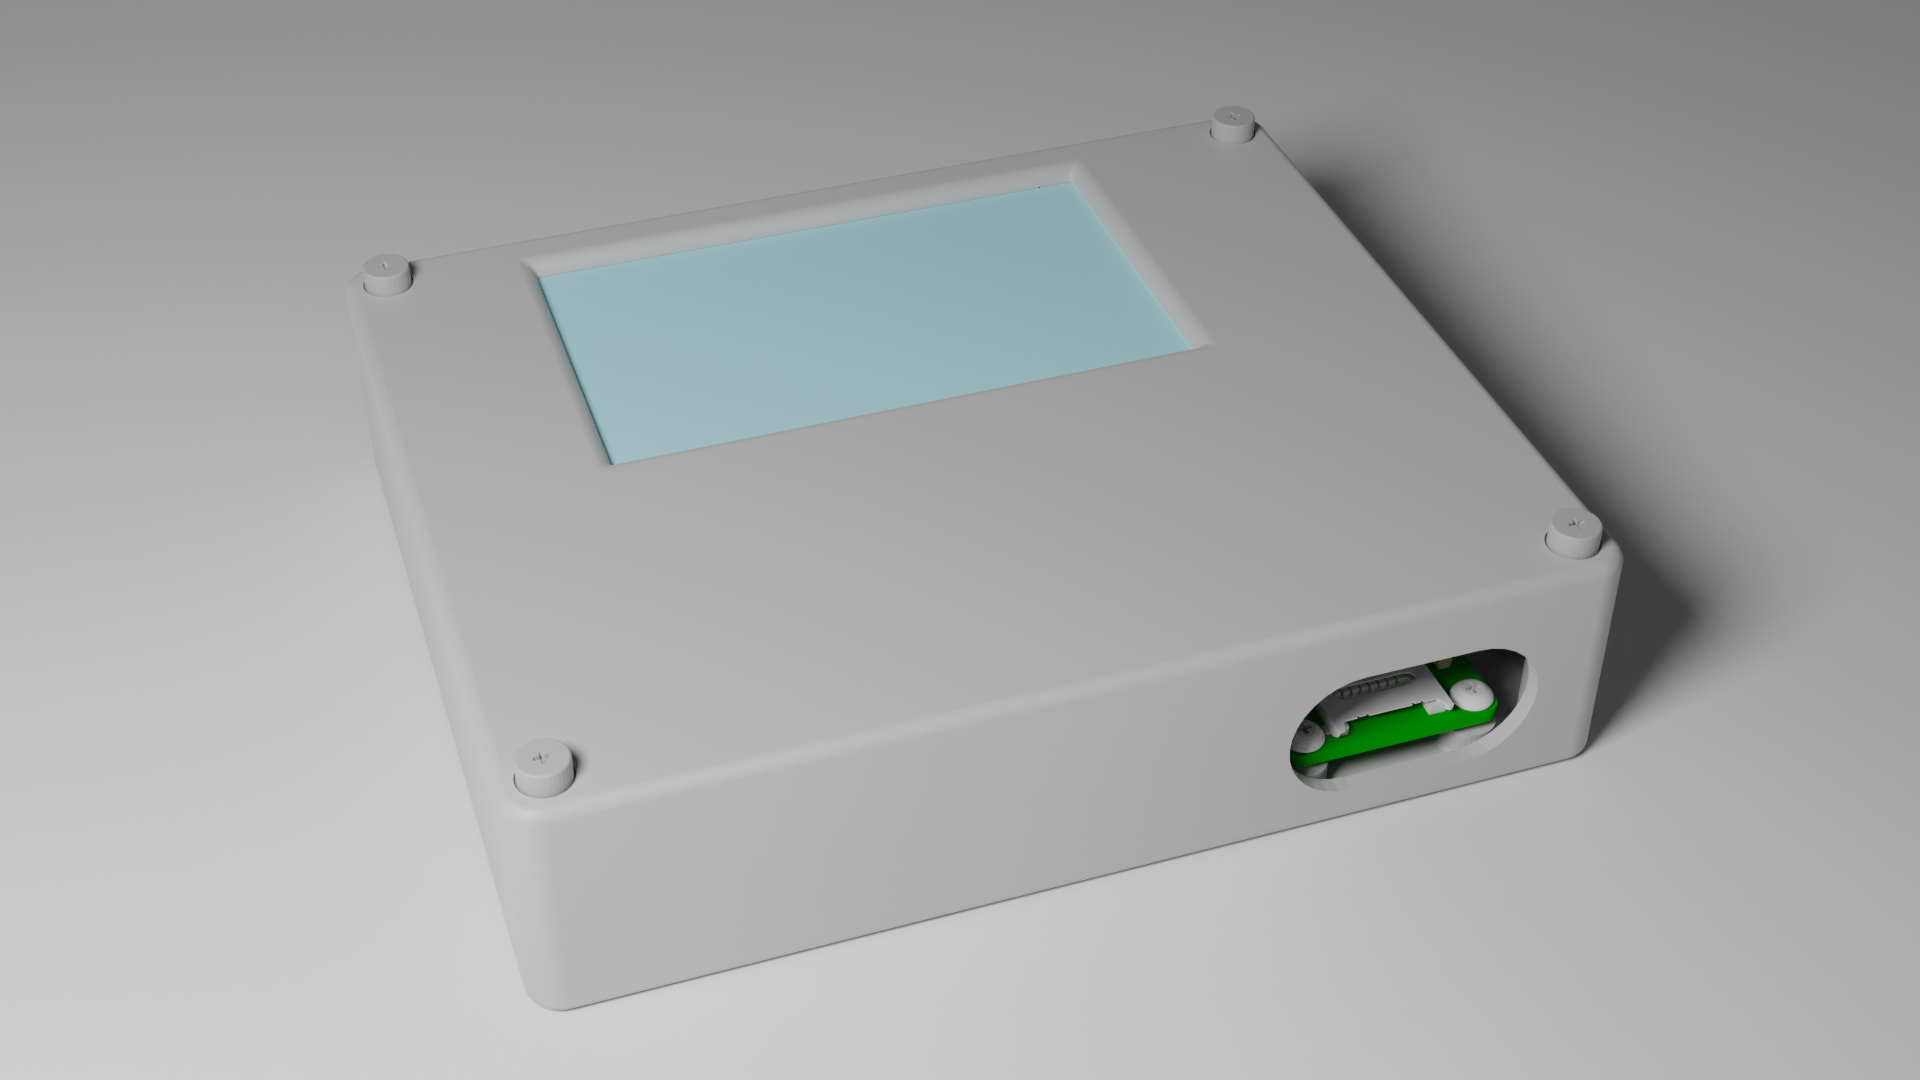
\includegraphics[width=\textwidth]{case_closed.png}
		\caption{Geschlossenes Gehäuse}
		\label{case_closed} 
	\end{subfigure}\\[5pt]%

\end{figure}

Um die Bedienung des Ein/Aus-Schalters zu vereinfachen wurde ein abgesetzter Zylinder konstruiert, der zwischen Platine und Gehäuse geklemmt wird. Der 3,5 mm Klinkenanschluss neben dem Schalter dient zum Anschließen der Elektrodenkabel (Abbildung \ref{case_no_display2}).